% BEGIN PREAMBEL
\documentclass[9pt]{beamer}
\usepackage[british]{babel}
\usepackage[latin1]{inputenc}
\usepackage{multimedia}
\usepackage{amsmath,amsfonts,amssymb}
\usepackage{upgreek}
\usepackage{pgfpages}
\usepackage[version=3]{mhchem}
\usepackage{lmodern}
\usepackage{graphicx}
\usepackage{multicol}
\usepackage{color}
\usepackage{xcolor}
\usepackage{wrapfig}
\usepackage{siunitx}
\usepackage{fontspec}
\newfontfamily\ubuntu{Ubuntu}
\newcommand{\as}{\\[14pt]}
\newcommand{\s}{\\[7pt]}
\newcommand{\is}{\\[2pt]}
\newcommand{\no}{\noindent}
\newcommand{\ka}{\hspace*{0.5cm}}
\newcommand{\ma}{\hspace*{1cm}}
\newcommand{\ga}{\hspace*{1.5cm}}
\newcommand{\li}{\left|}
\newcommand{\re}{\right|}
\newcommand{\const}{\text{const.}}
\newcommand{\z}{\text}
\newcommand{\terminal}[1]{\colorbox{black}{\textcolor{white}{{\fontfamily{phv}\selectfont \scriptsize{#1}}}}}
\newcommand{\plugin}[1]{\textit{\flq#1\frq}}
\definecolor{darkcerulean}{rgb}{0.03, 0.27, 0.49}
\newcommand{\ubu}[1]{{\color{darkcerulean}\footnotesize \ubuntu #1}}
\usetheme{Boadilla}
\graphicspath{ {Pics/} }
\usecolortheme{beaver}
\useoutertheme{miniframes}
\beamertemplatenavigationsymbolsempty
\makeindex
\title[Analysis]{Discussion of the Pad Analysis}
\author[M. Reichmann]{Michael Reichmann}
\institute[\textbf{\textit{ETH}}\scalebox{.6}{\textit{Z\"{u}rich}}]{Swiss Federal Institute of Technology Zurich}
\AtBeginSection{\frame{\sectionpage}}
% END PREAMBEL
\begin{document}
% ============================
% BEGIN TITLE PAGE
% ============================
\begin{frame}
	\begin{center}
		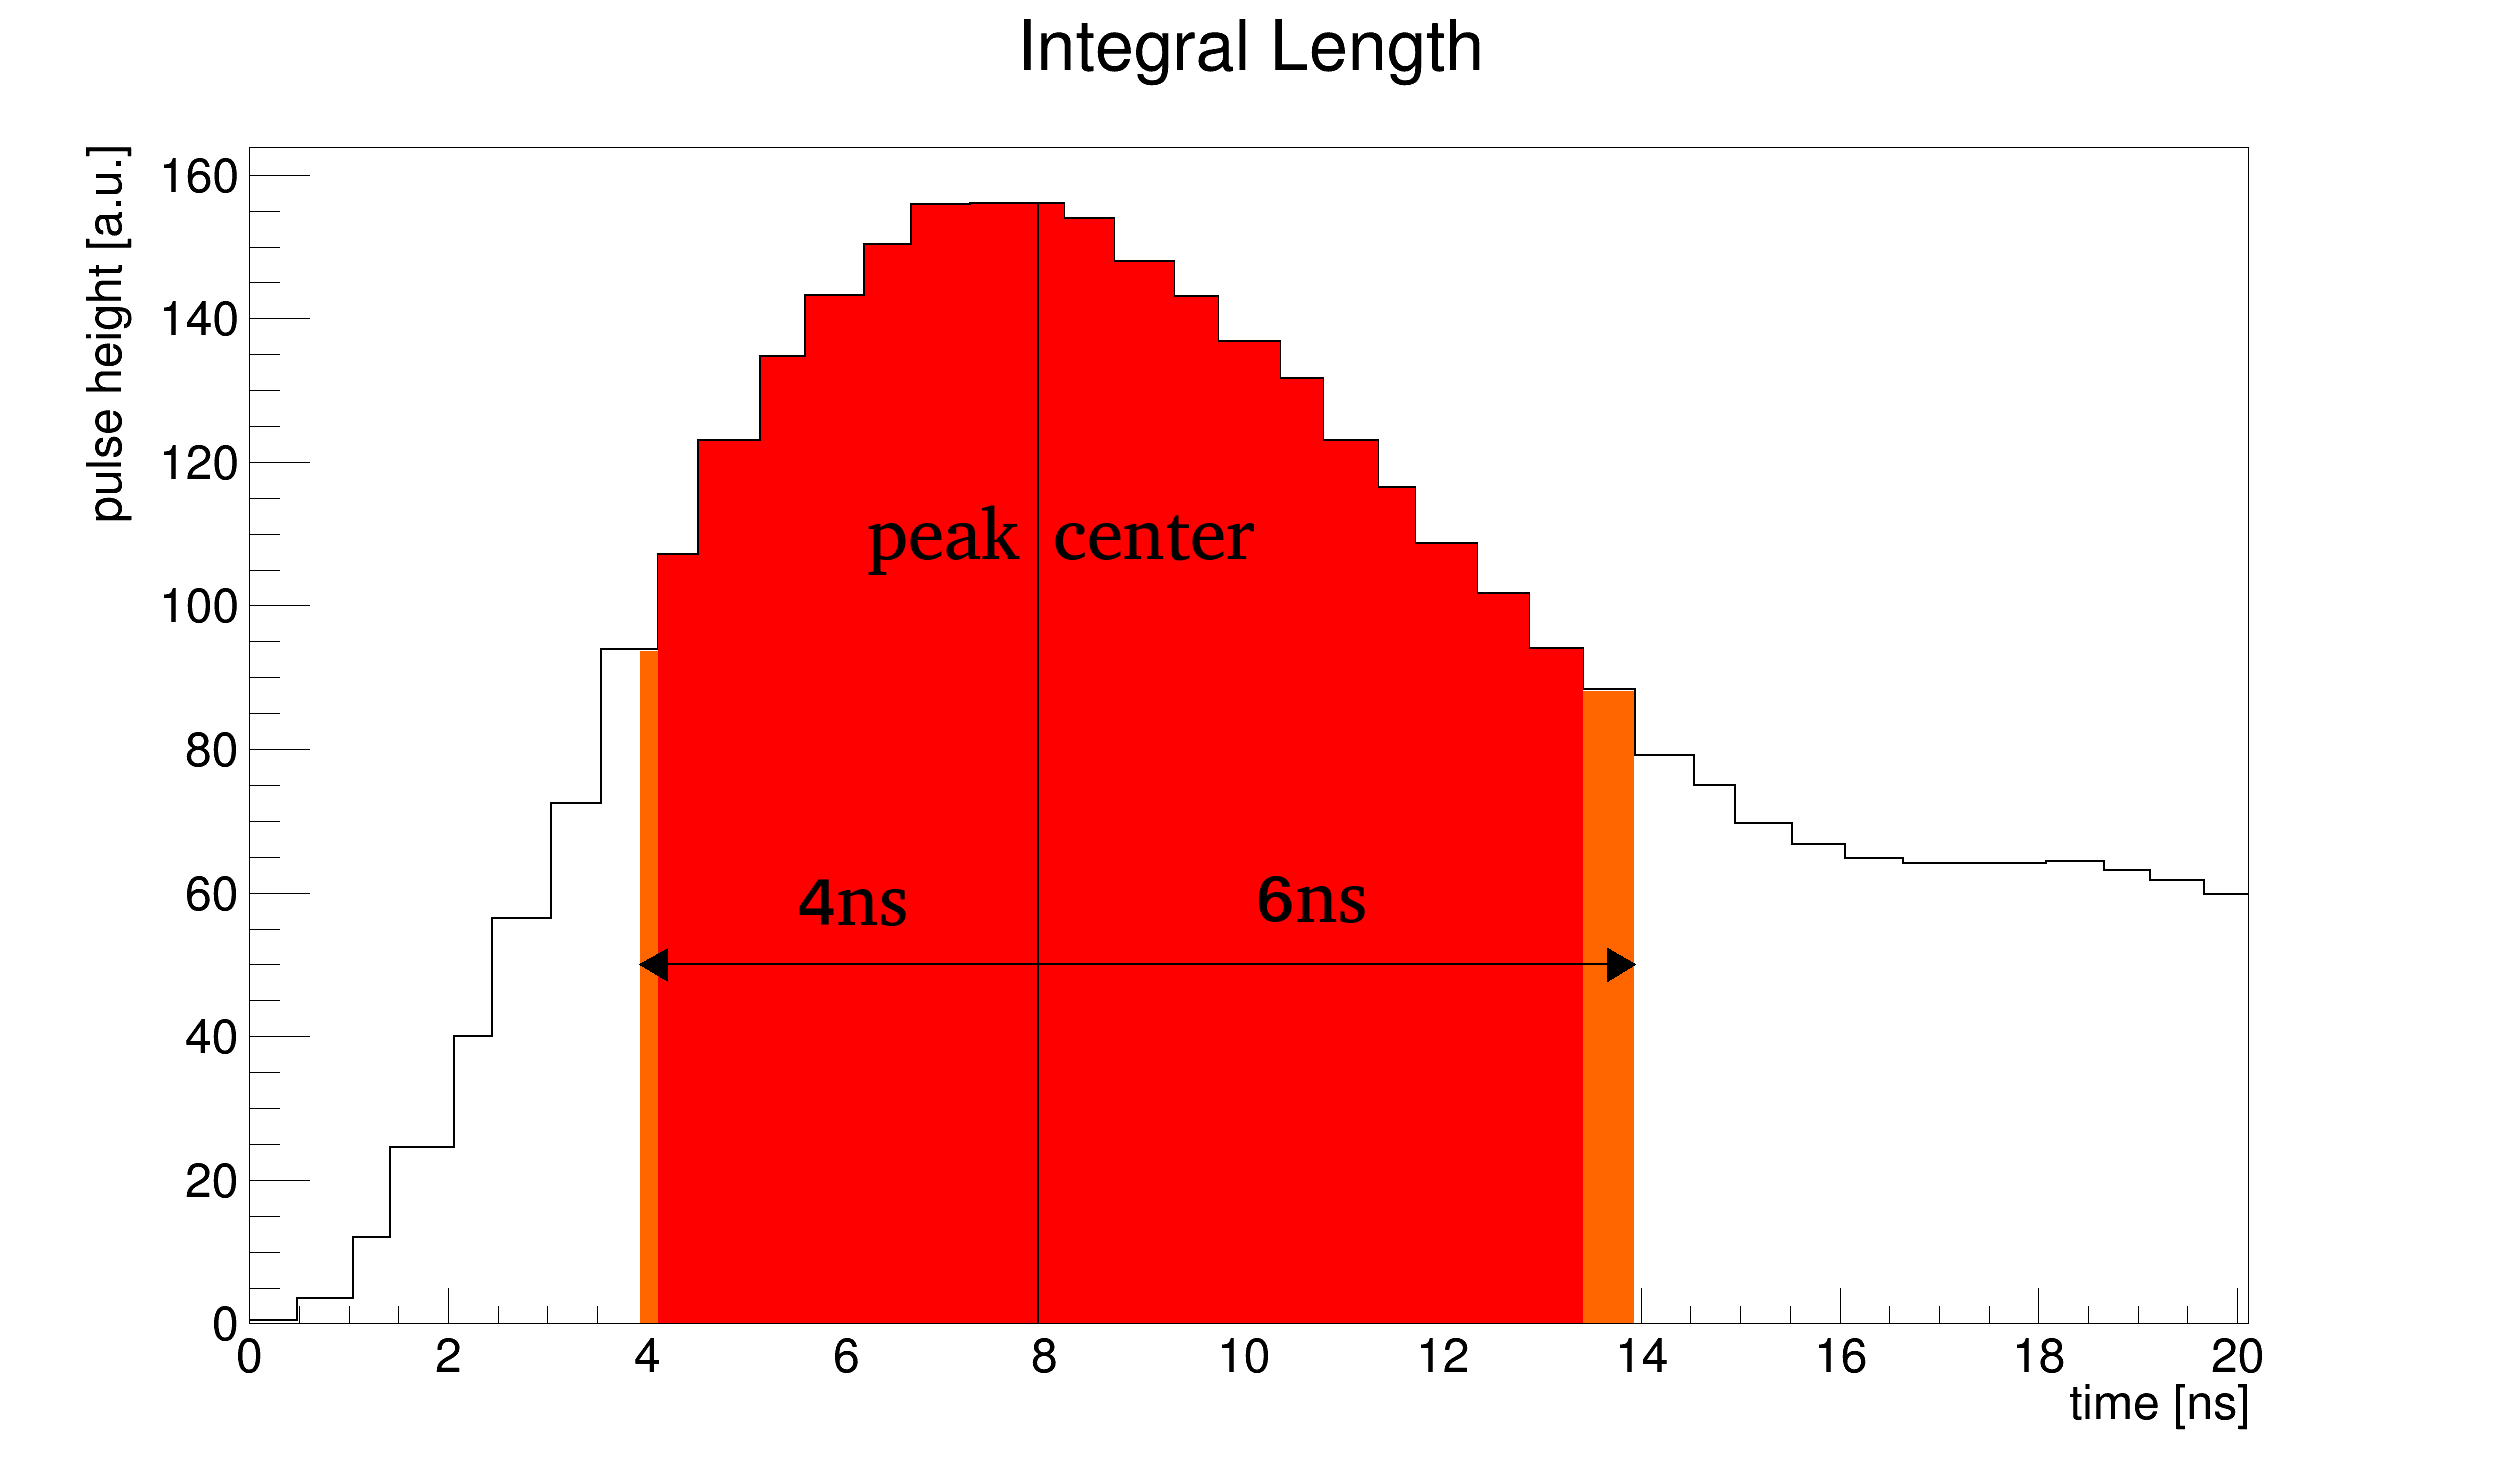
\includegraphics[width=6cm]{IntegralLength}
	\end{center}
	\begin{alertblock}{
		\begin{center}
			\textbf{Meeting \today}
		\end{center}}
		\vspace*{10pt}
		\begin{center}\small
		Speaker: Felix Bachmair
		\end{center}\normalsize
	\end{alertblock}
\end{frame}
% END
% ============================
% BEGIN TABLE OF CONTENTS
% ============================
\begin{frame}[allowframebreaks]
	\frametitle{Table of contents}
	\tableofcontents   % [pausesections]
\end{frame}
% END
% ====================================================================================
% BEGIN TRIGGER CELL
% ====================================================================================
\section{DRS4 Cells}
% ============================
\subsection{Cell Length}
\begin{frame}
	\begin{center}
		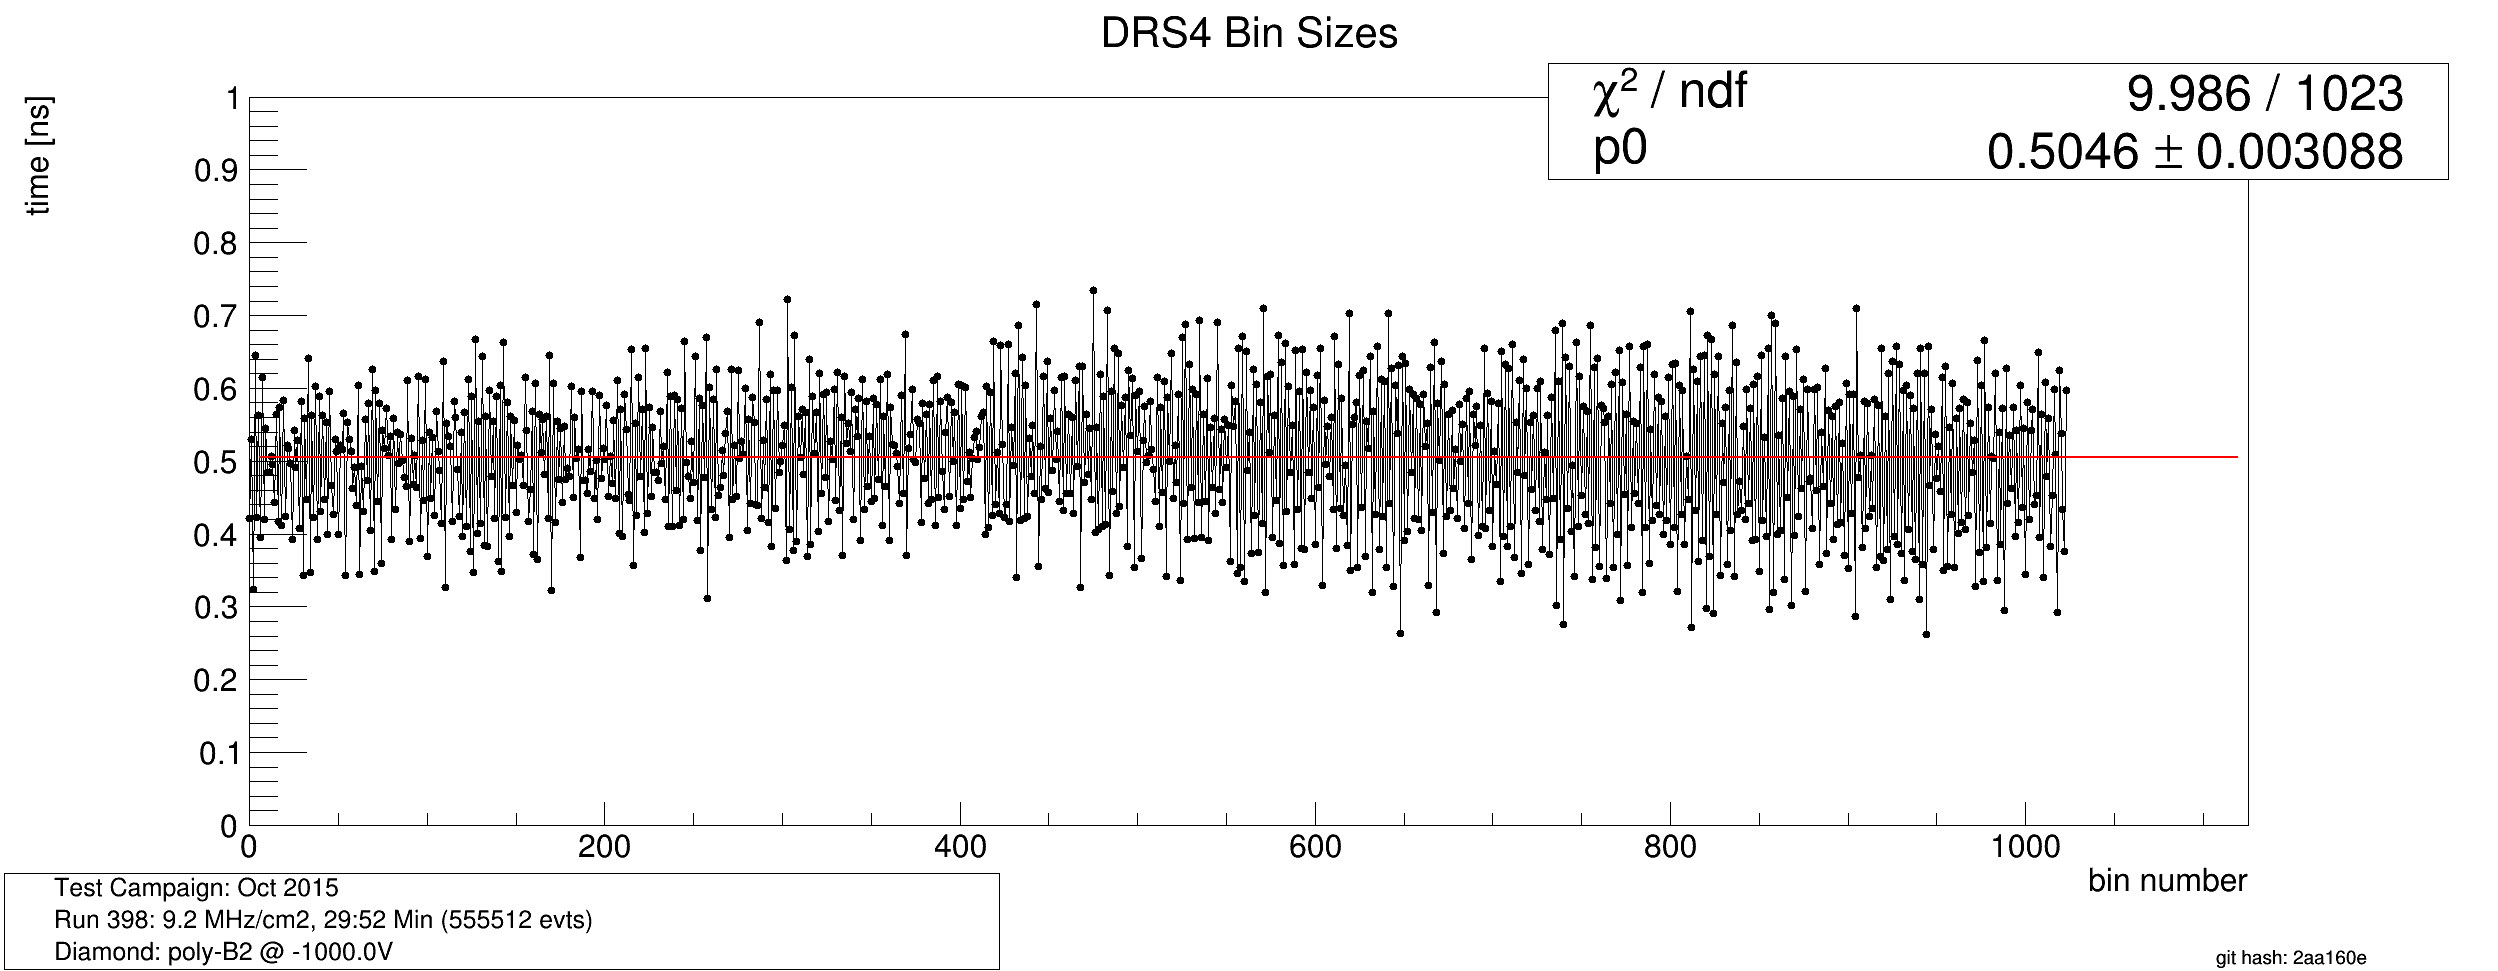
\includegraphics[width=11cm]{DRSBinSizes}
	\end{center}
	\begin{minipage}{3.5cm}
		\centering
		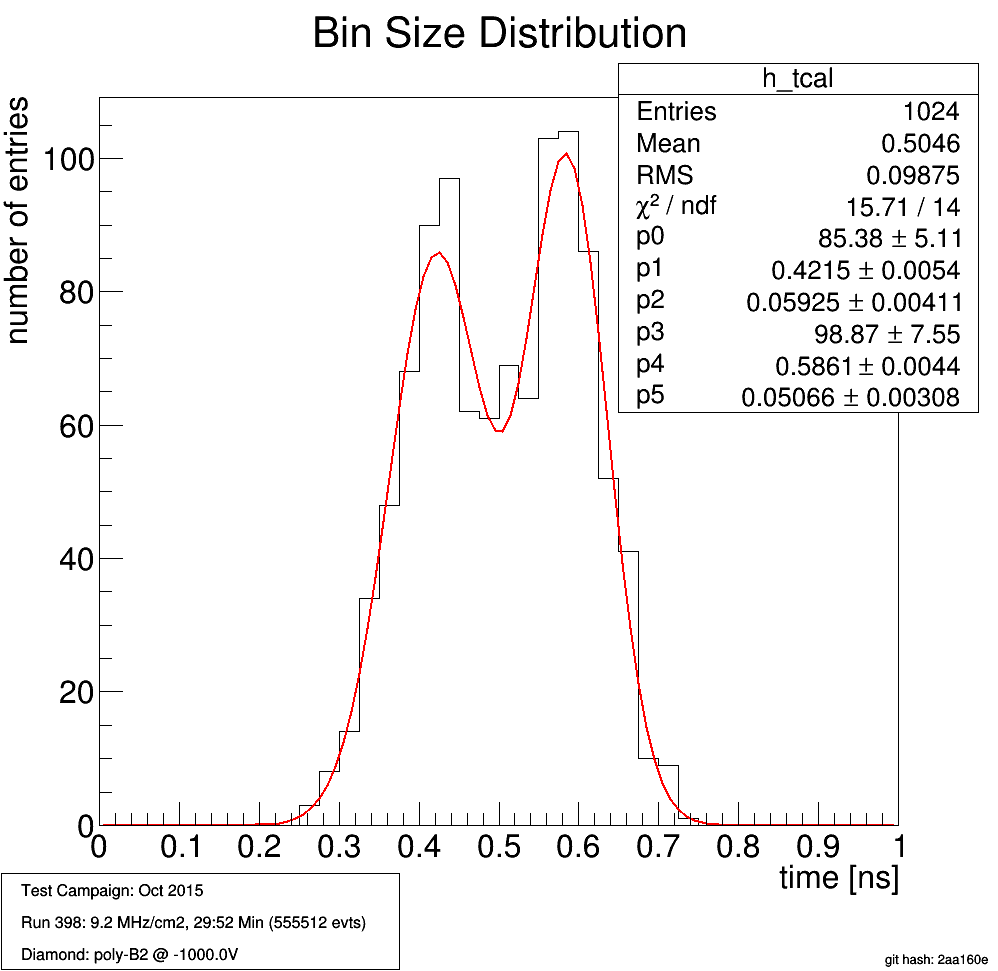
\includegraphics[width=3.5cm]{BinDisto}
	\end{minipage}
	\hspace*{2pt}
	\begin{minipage}{7.5cm}
		\begin{itemize}
			\item bin sizes centered around .5
			\item two gaussian peaks around \SI{.42}{ns} and \SI{.59}{ns} with sigmas of $\approx$ \SI{.05}{ns}
		\end{itemize}
	\end{minipage}
\end{frame}
% new frame ============================
% END
% ====================================================================================
% BEGIN INTEGRAL LENGTH
% ====================================================================================
\section{Signal Vs. Trigger Cell}
% ============================
\subsection{Fixed Bins}
\begin{frame}
	\begin{center}
		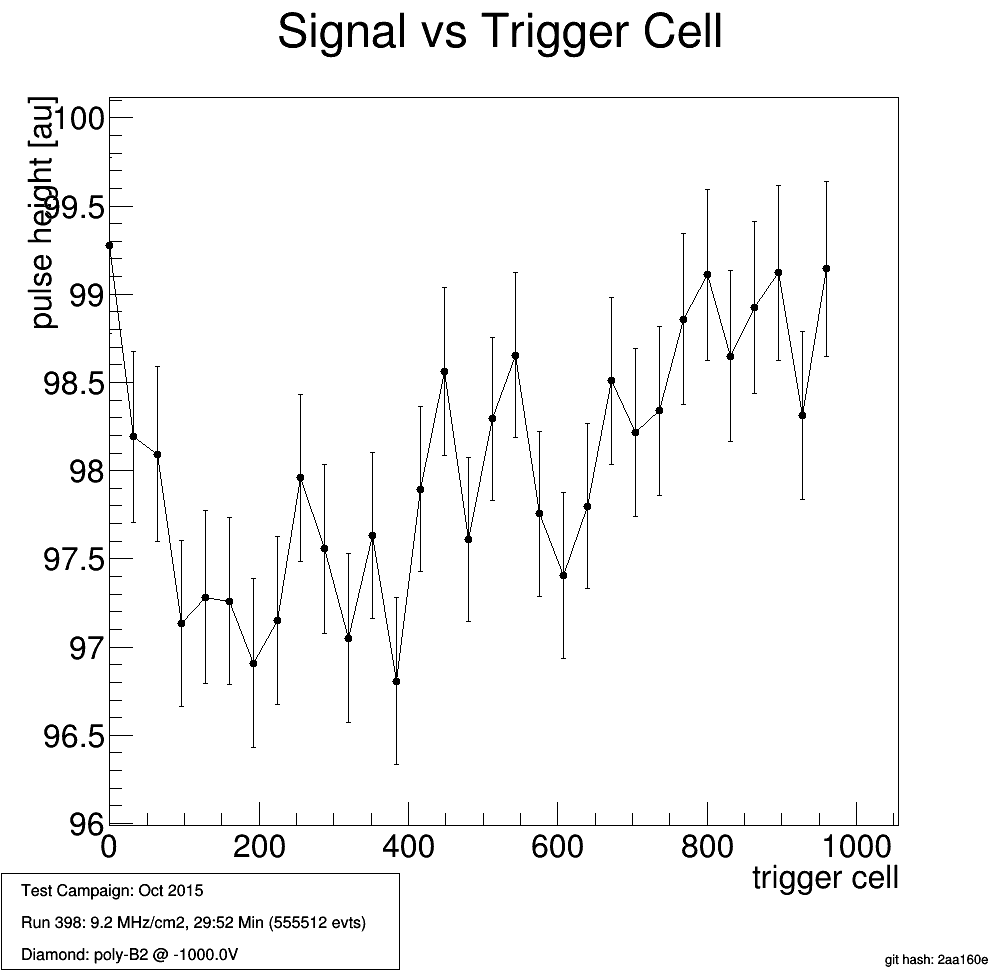
\includegraphics[width=6cm]{SignalVsTriggerCell}
	\end{center}
	\begin{itemize}
		\item using fixed bin size for the integration
		\begin{itemize}
			\item length of integral depending on trigger cell since bins have different sizes
		\end{itemize}
	\end{itemize}
\end{frame}
% ============================
\subsection{Fixed Time}
\begin{frame}
	\begin{center}
		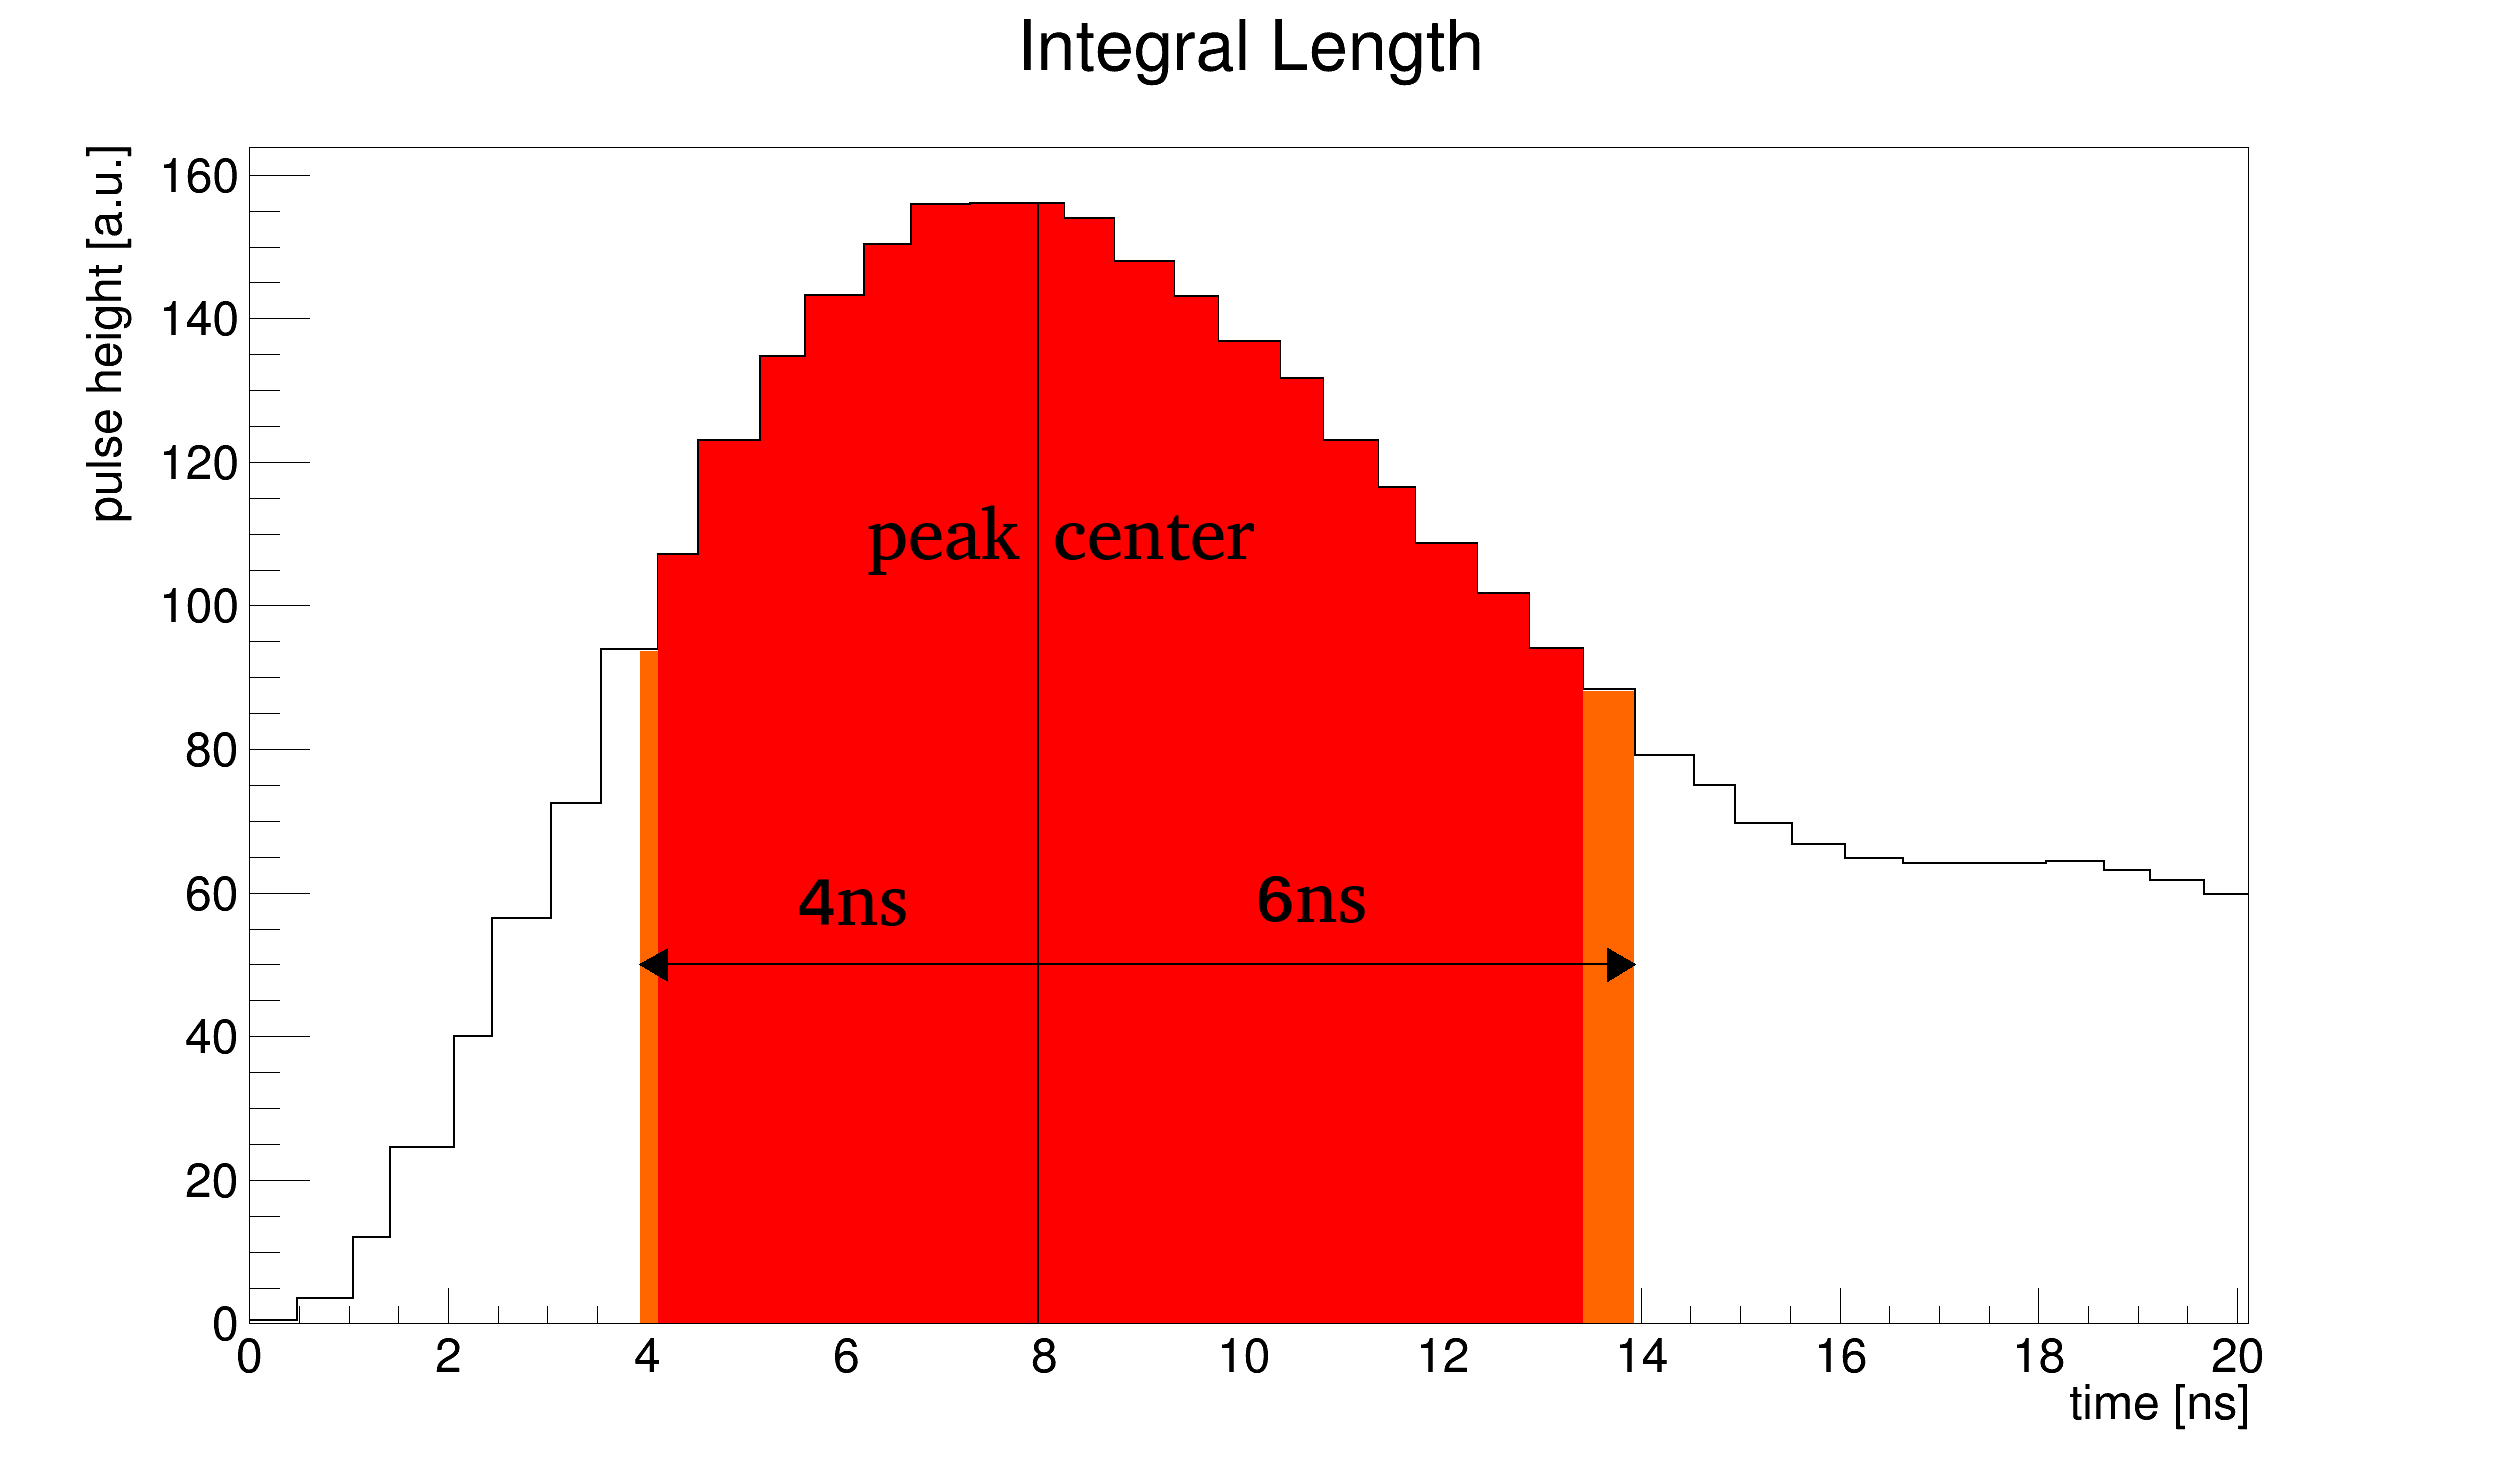
\includegraphics[width=8cm]{IntegralLength}
	\end{center}
	\begin{itemize}
		\setlength{\itemsep}{\fill}
		\item different time sizes of the bins
		\item using same interval as before: [8,12] $\rightarrow$ [\SI{4}{ns}, \SI{6}{ns}] taking \SI{.5}{ns} as average bin size
		\item summing up the pulse heights until the integral has a fixed time size
		\item taking part of the outer bins (orange) that is missing to the exact time value
		\item use straight line approximation?
		\item $\rightarrow$ make new SNR study!
	\end{itemize}
\end{frame}
% new frame ===================
\begin{frame}
	\begin{minipage}{5.5cm}
		\centering
		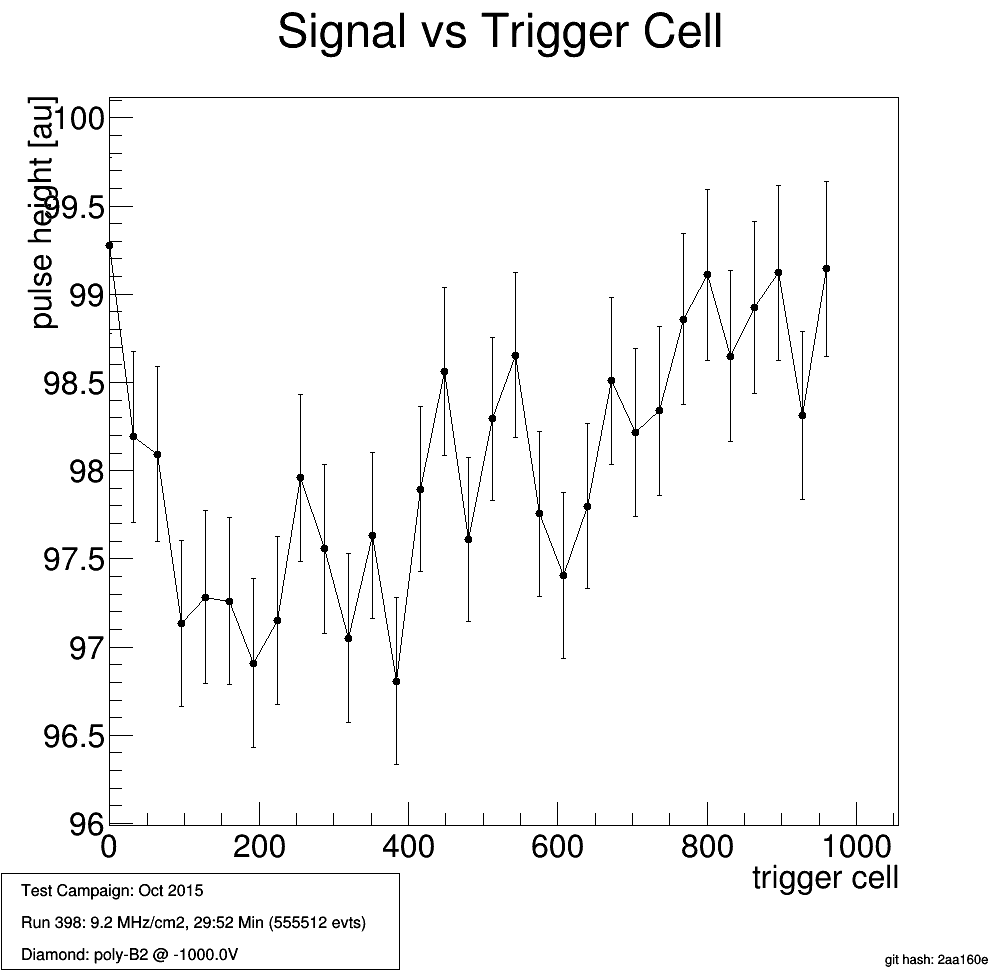
\includegraphics[width=5.5cm]{SignalVsTriggerCell}
	\end{minipage}
	\hspace*{2pt}
	\begin{minipage}{5.5cm}
		\centering
		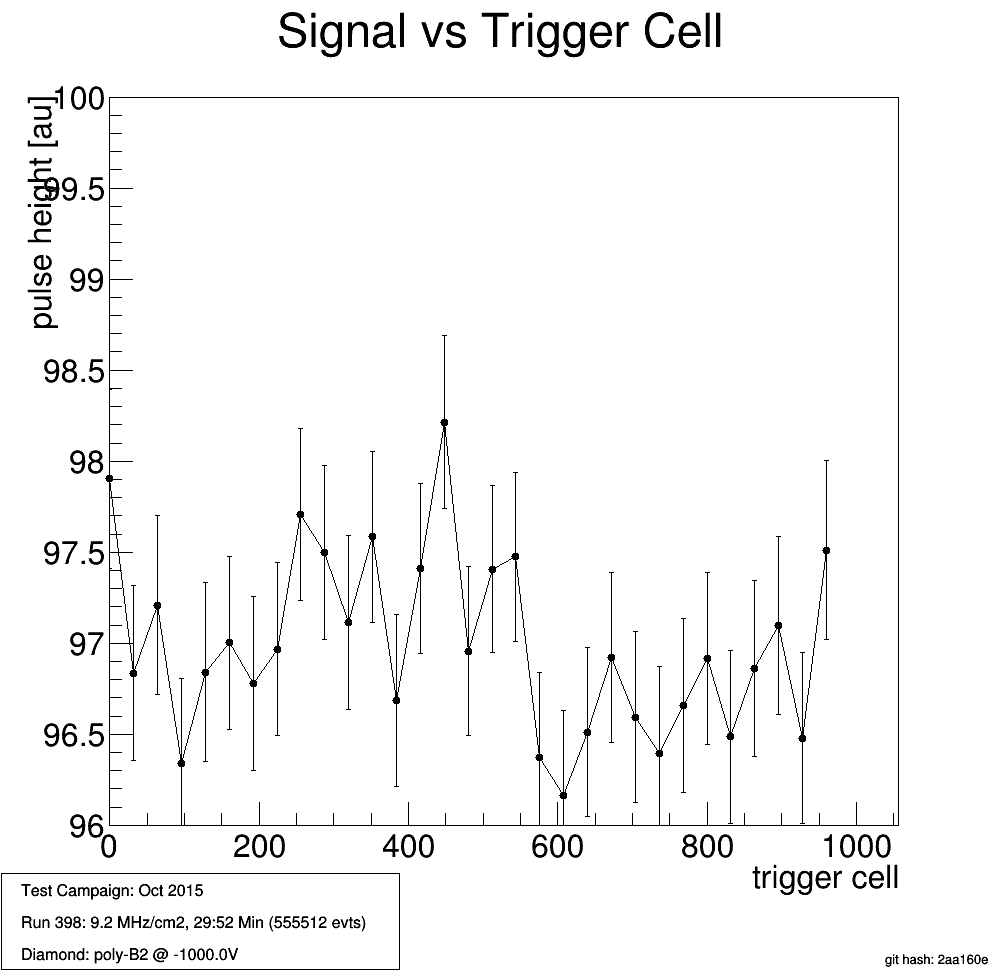
\includegraphics[width=5.5cm]{SignalVsTrig}
	\end{minipage}\s
	\begin{itemize}
		\item using fixed time integral length flattens the behaviour of the pulse heights
		\item $\upchi^{2}$: $78/26$ with \SI{30}{dof} of pol0 fit
	\end{itemize}
\end{frame}
% END
% ====================================================================================
% BEGIN TIMING CUT
% ====================================================================================
\section{Peak Timing Cut}
% ============================
\subsection{Peak Timing Vs Trigger Cell}
\begin{frame}
	\begin{center}
		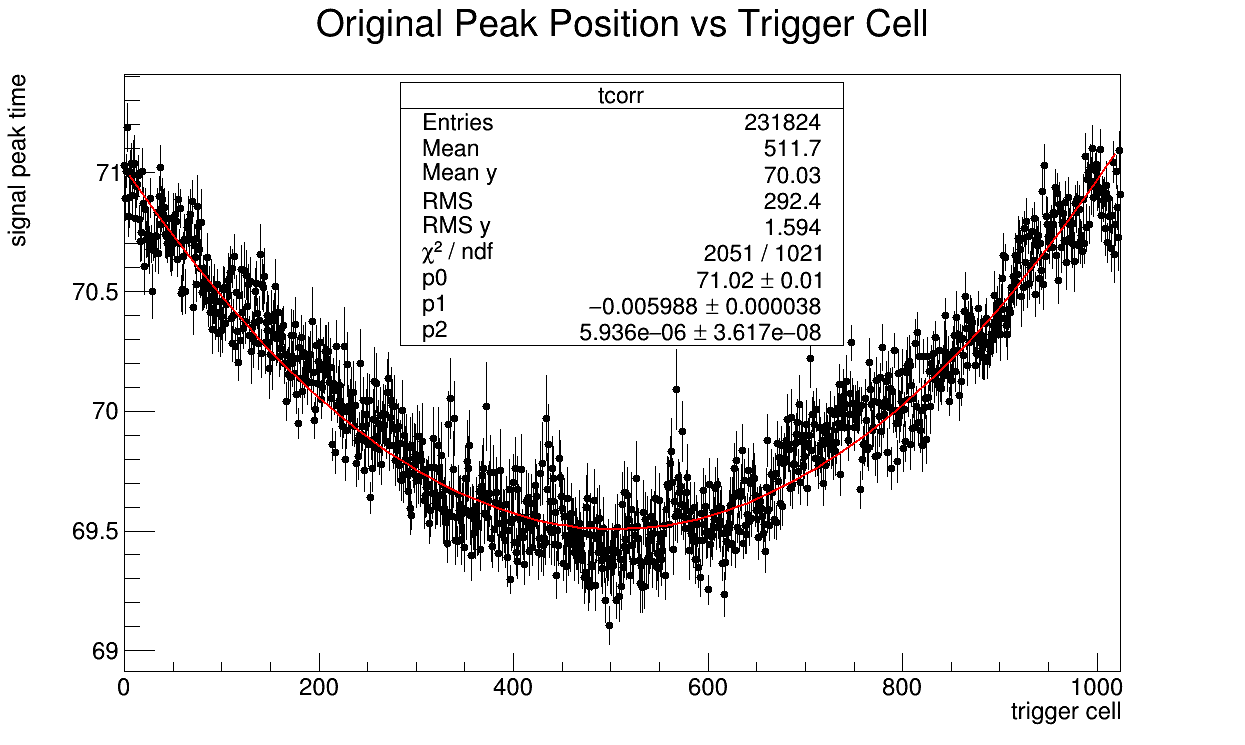
\includegraphics[width=8cm]{PeakTimeVsTrigCell}
	\end{center}
	\begin{itemize}
		\item still slight dependence on the trigger cell
		\item introducing trigger cell dependent cut based on the pol2 fit
		\begin{itemize}
			\item TMath::Abs(Signal - p1 * trigger\_cell - p2 * trigger\_cell * trigger\_cell) - mean) / sigma < 3
		\end{itemize}
		\item takes out all events that are not in between $3$ sigma of the corrected peak timings
	\end{itemize}
\end{frame}
% ============================
\subsection{Sigma}
\begin{frame}
	\begin{center}
		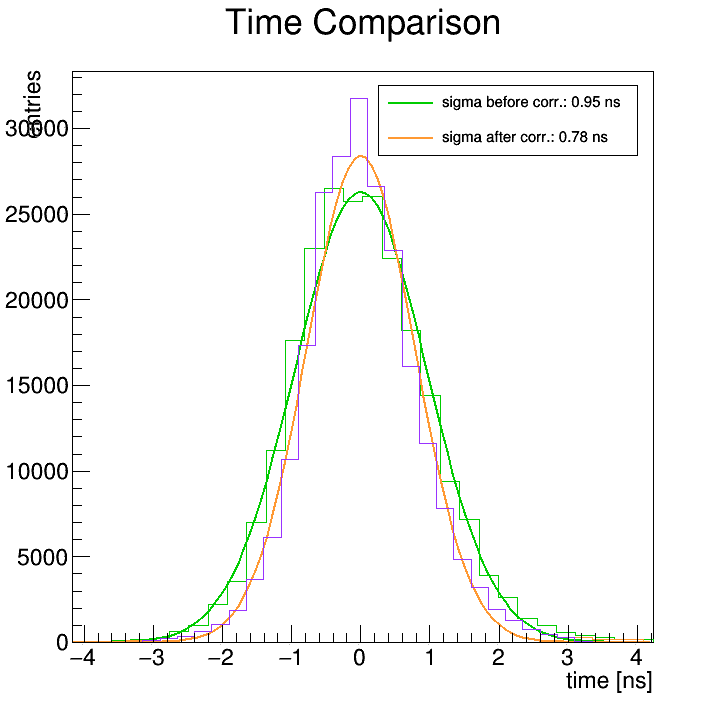
\includegraphics[width=6cm]{TimeComparison.png}
	\end{center}
	\begin{itemize}
		\item \SI{0.78}{ns} time resolution after the correction!!
		\item \textbf{hier waere dein Plot mit der region auf wir cutten noch toll!!}
	\end{itemize}
\end{frame}
% END
% ====================================================================================
% BEGIN PEAK POSITIONS
% ====================================================================================
\section{Peak Positions}
% ============================
\subsection{Peak Positions}
\begin{frame}
	\begin{center}
		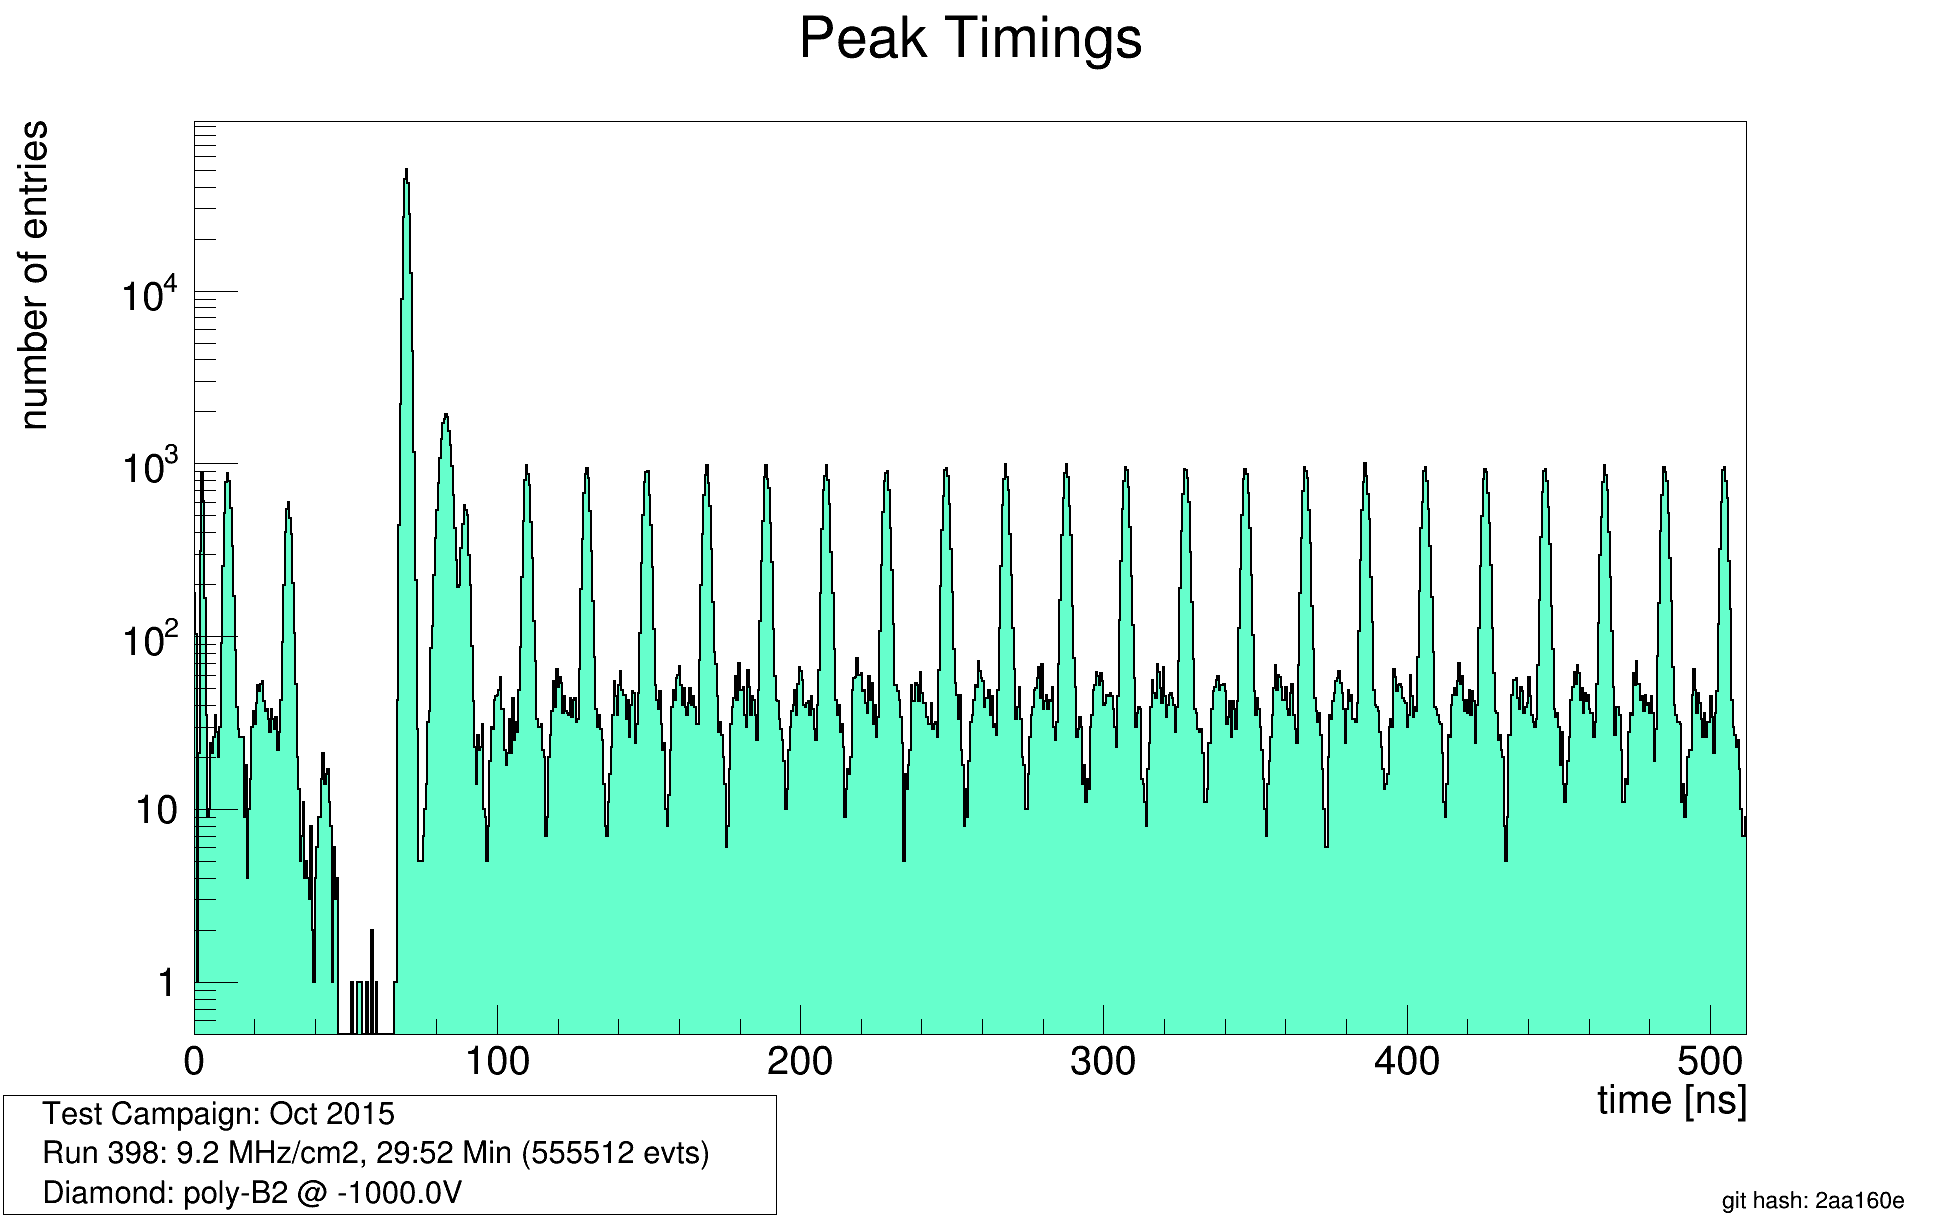
\includegraphics[width=8cm]{PeakTimings}
	\end{center}
	\begin{itemize}
		\item highest peak = trigger peak
		\item secondary peak completeley evenly distributed $\rightarrow$ nice poissonian beam
		\item peaks in between the secondary peaks
		\begin{itemize}
			\item almost same ratio of trigger peak/peak after as secondary peaks/peak in between
			\item idea different particle type! (positrons, myons?)
			\item possibility to trigger on other particles
		\end{itemize}
	\end{itemize}
\end{frame}
% ============================
\subsection{Peak Numbers}
\begin{frame}
	\begin{minipage}{5.5cm}
		\centering
		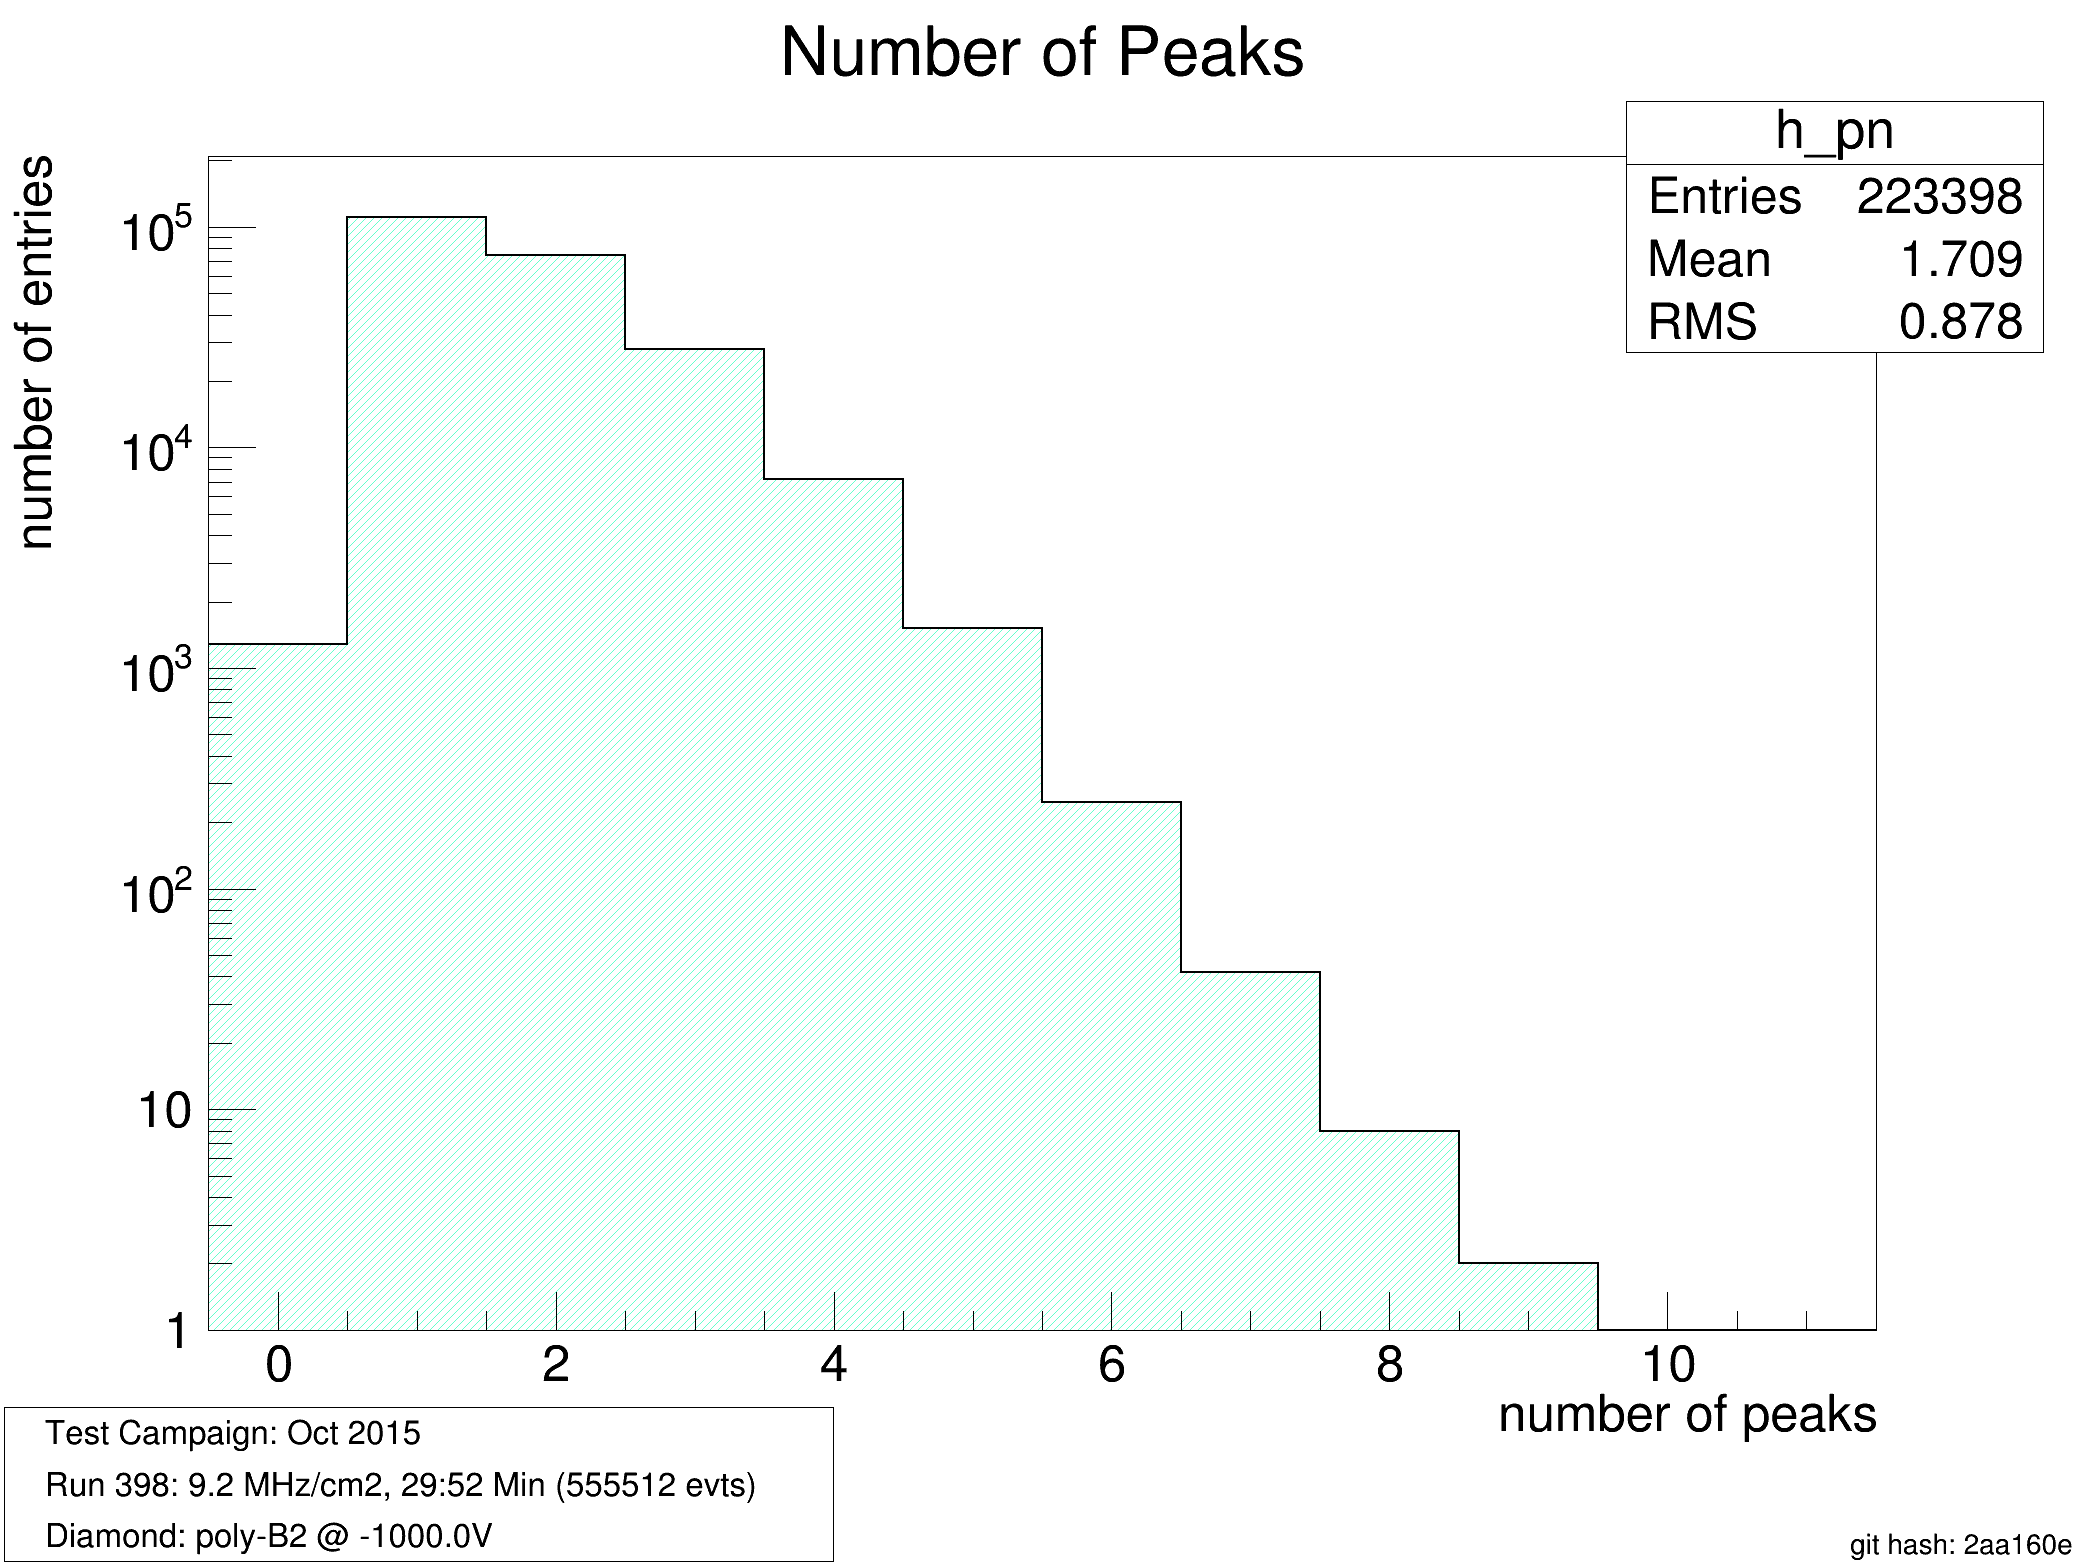
\includegraphics[width=5.5cm]{PeakNumbers}
	\end{minipage}
	\hspace*{2pt}
	\begin{minipage}{5.5cm}
		\centering
		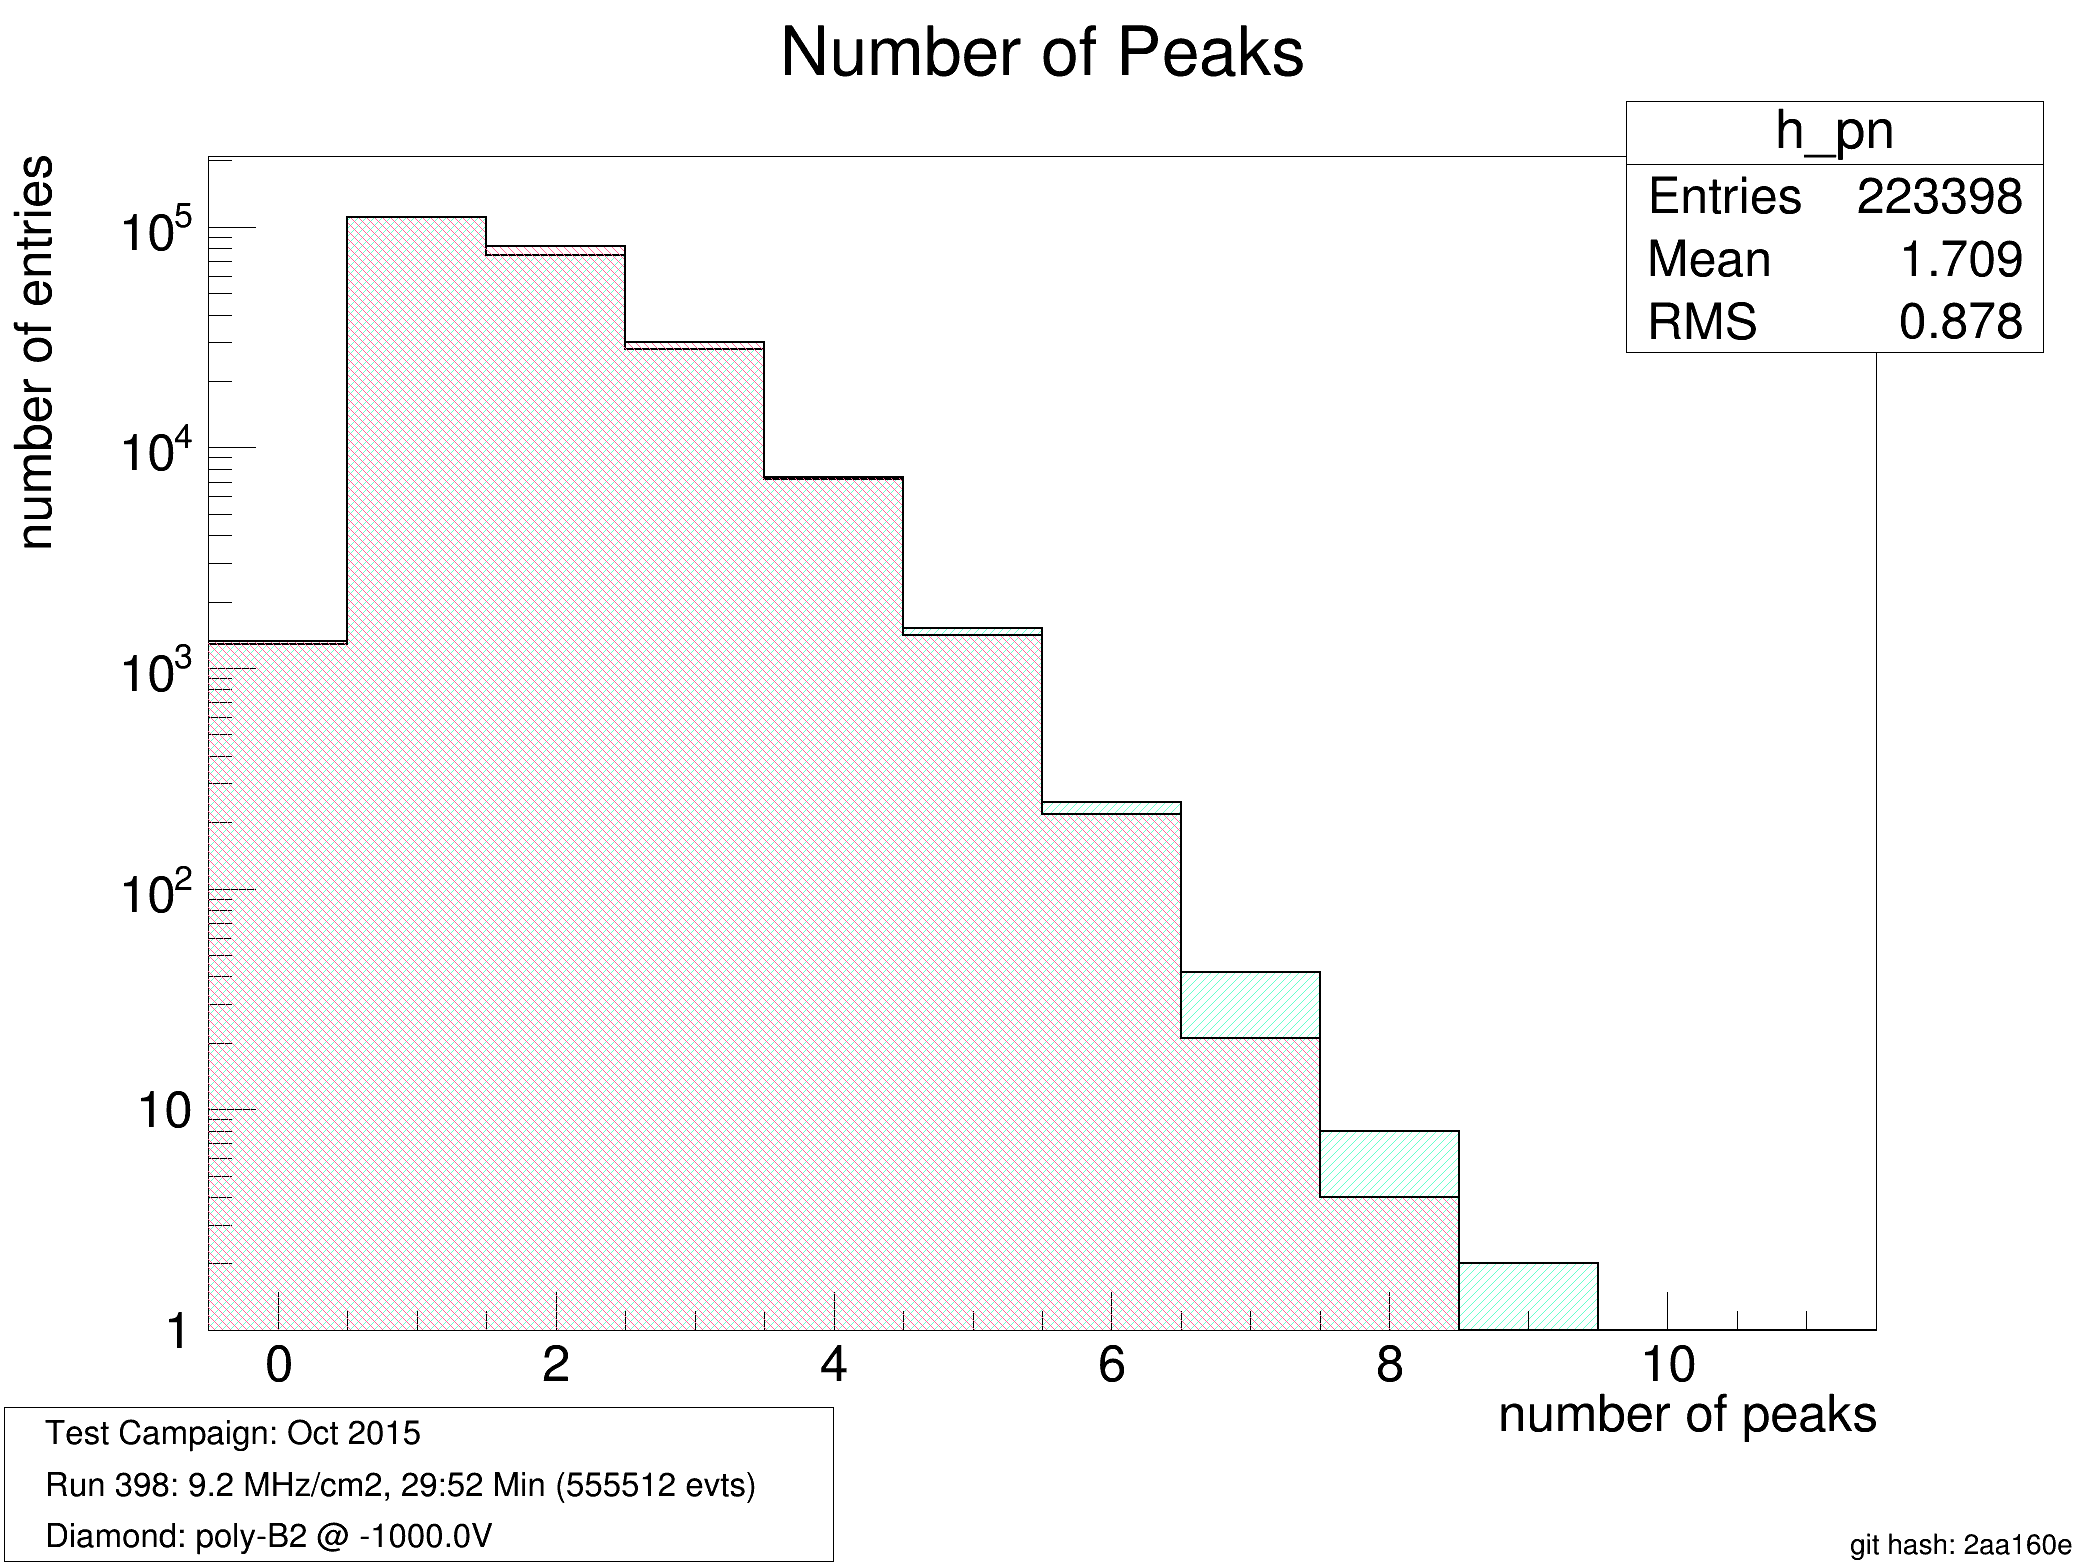
\includegraphics[width=5.5cm]{PeakNumbersEst}
	\end{minipage}\s
	\begin{itemize}
		\item pink distribtion histo filled with \ubu{gRandom.Poisson(24 * self.get\_flux() / 5e4 * .5 * .5 * p2) + gRandom.Binomial(1, p1)}
		\begin{itemize}
			\item p1 = 0.988, p2 = 0.68
		\end{itemize}
		\item measured flux has the correct order of magnitude
		\item use distribution to estimate the flux!?
		\begin{itemize}
			\item does it mean that flux is 68\% lower than expected?
			\item longer tail due to peak of additional particles?
			\item wrong size of the diamond // edges less efficiant?
			\item influence of dead time?
		\end{itemize}

	\end{itemize}
\end{frame}
% ============================
% END
% ====================================================================================
% BEGIN AUGUST DATA
% ====================================================================================
\section{August 2015 Beam Test Data}
% ============================
\subsection{Poly B2}
\begin{frame}
	\frametitle{\SI{-1000}{V}}
	\begin{minipage}{5.5cm}
		\centering
		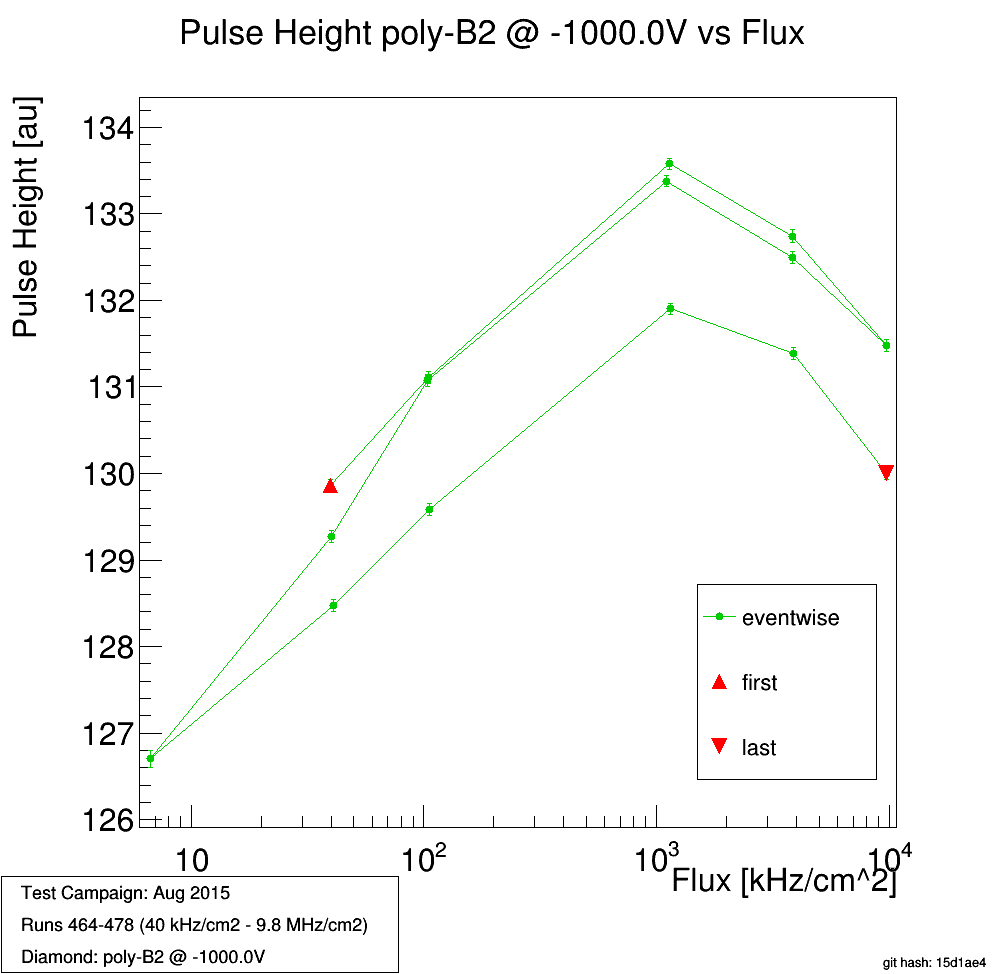
\includegraphics[width=5.5cm]{PhB2Neg}
	\end{minipage}
	\vspace*{2pt}
	\begin{minipage}{5.5cm}
		\centering
		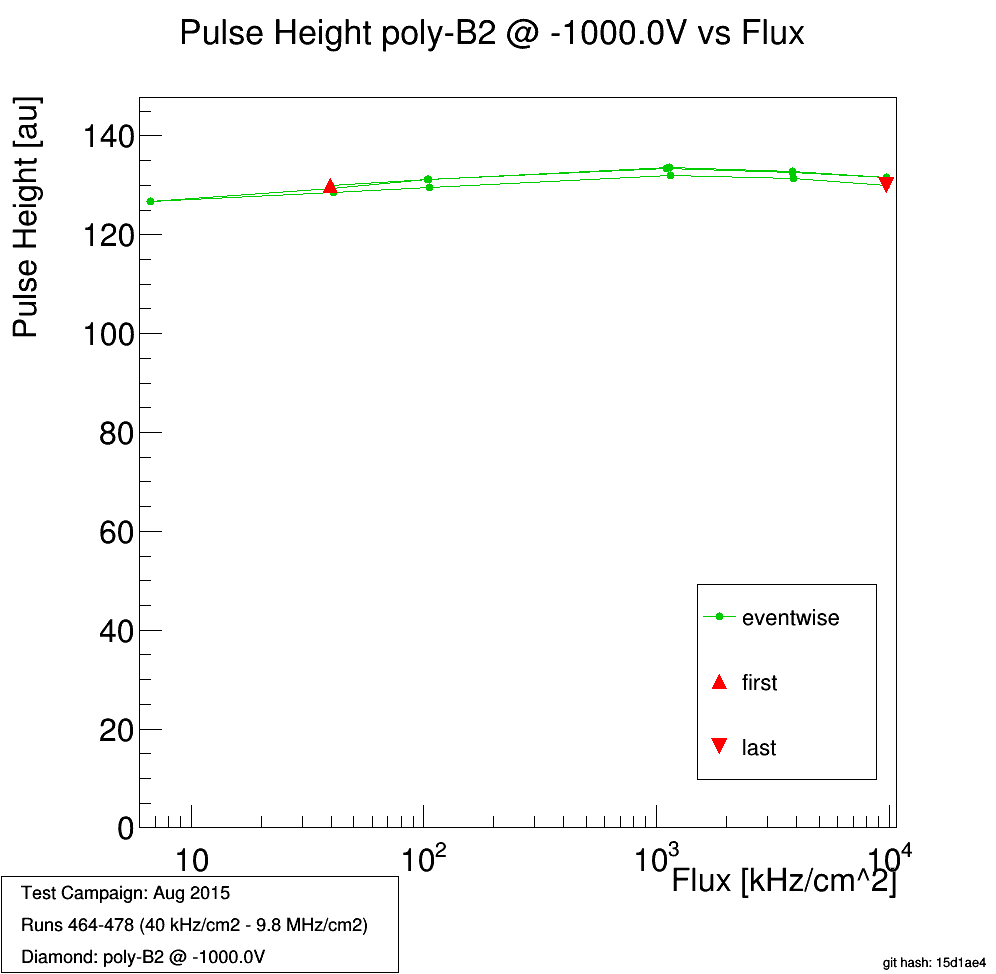
\includegraphics[width=5.5cm]{PhB2NegZero}
	\end{minipage}
\end{frame}
% new frame===================
\begin{frame}
	\frametitle{+\SI{1000}{V}}
	\begin{minipage}{5.5cm}
		\centering
		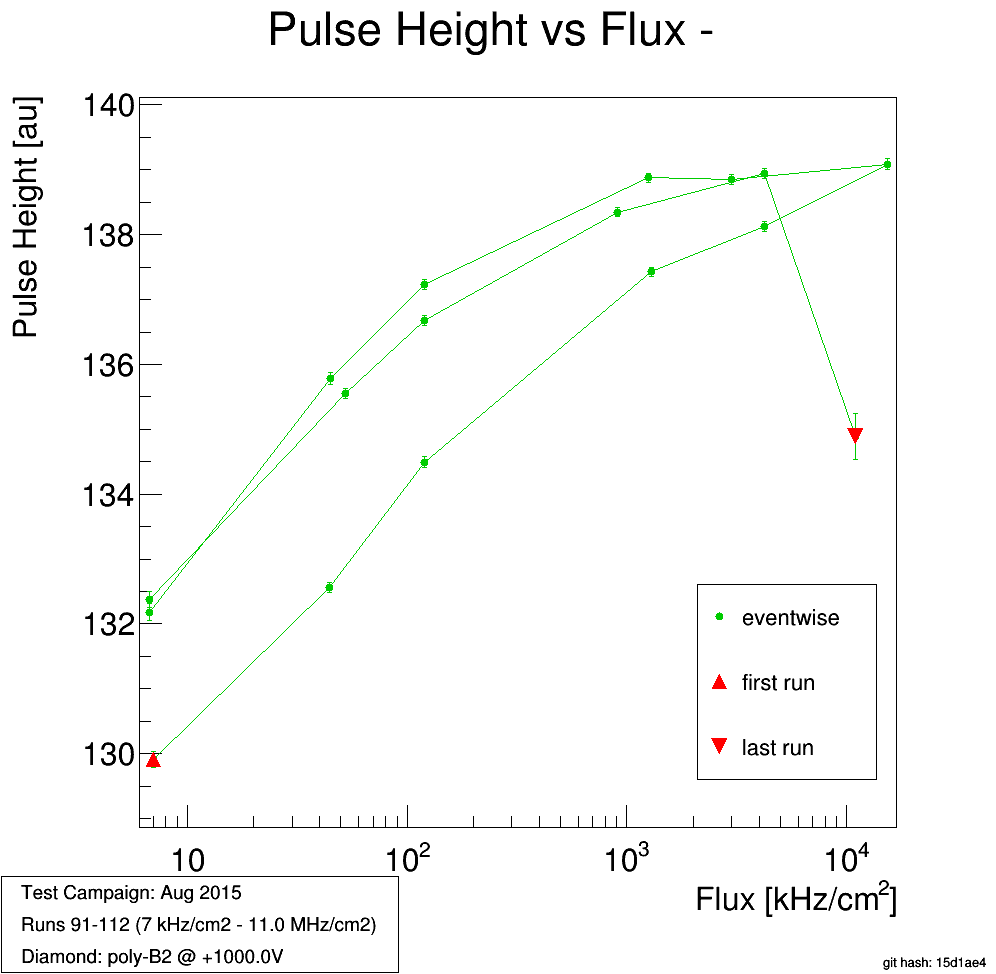
\includegraphics[width=5.5cm]{PhB2Pos}
	\end{minipage}
	\vspace*{2pt}
	\begin{minipage}{5.5cm}
		\centering
		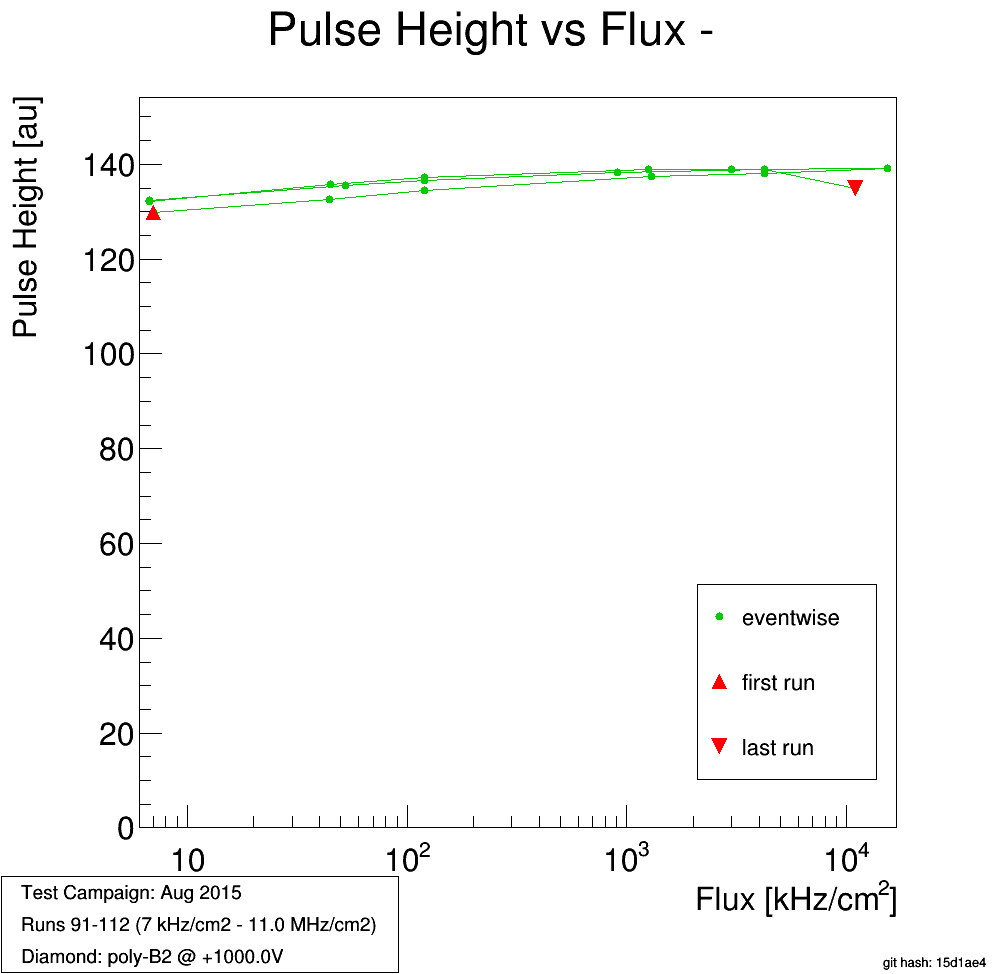
\includegraphics[width=5.5cm]{PhB2PosZero}
	\end{minipage}
\end{frame}
% ============================
\subsection{S129}
\begin{frame}
	\frametitle{\SI{-500}{V}}
	\begin{minipage}{5.5cm}
		\centering
% 		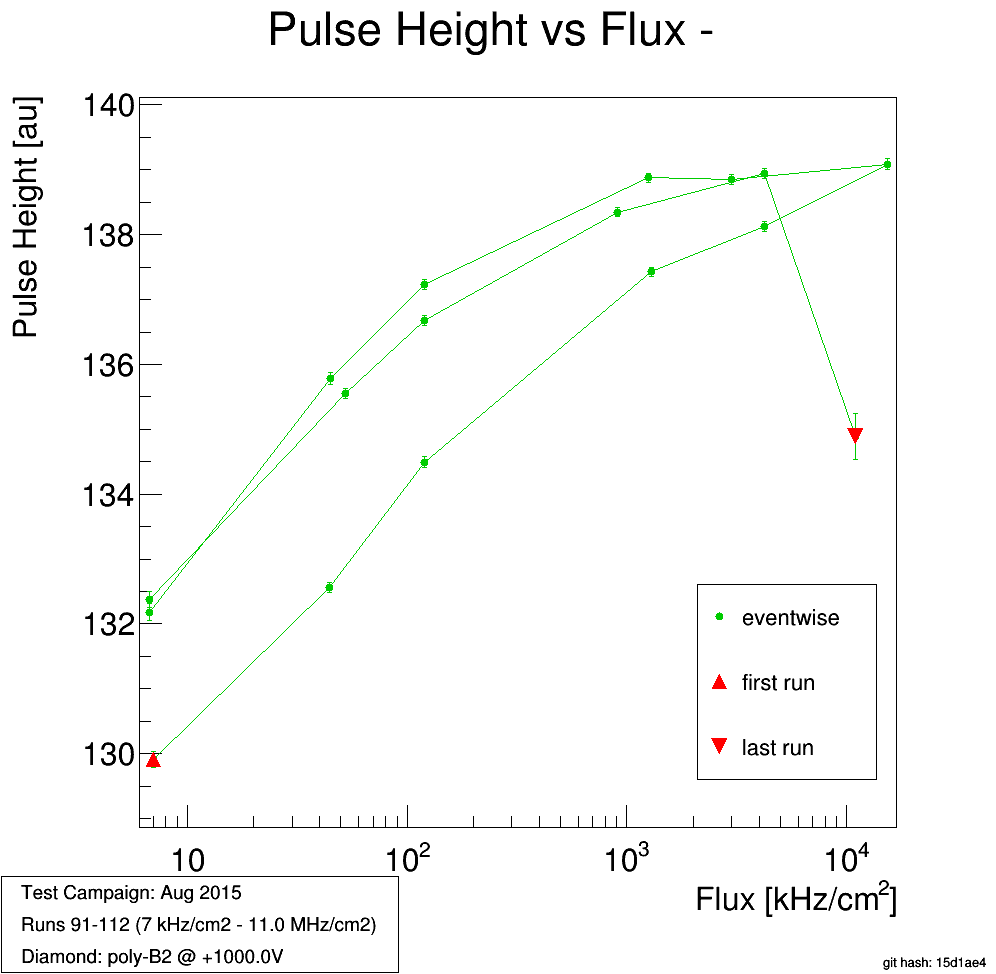
\includegraphics[width=5.5cm]{PhB2Pos}
	\end{minipage}
	\vspace*{2pt}
	\begin{minipage}{5.5cm}
		\centering
% 		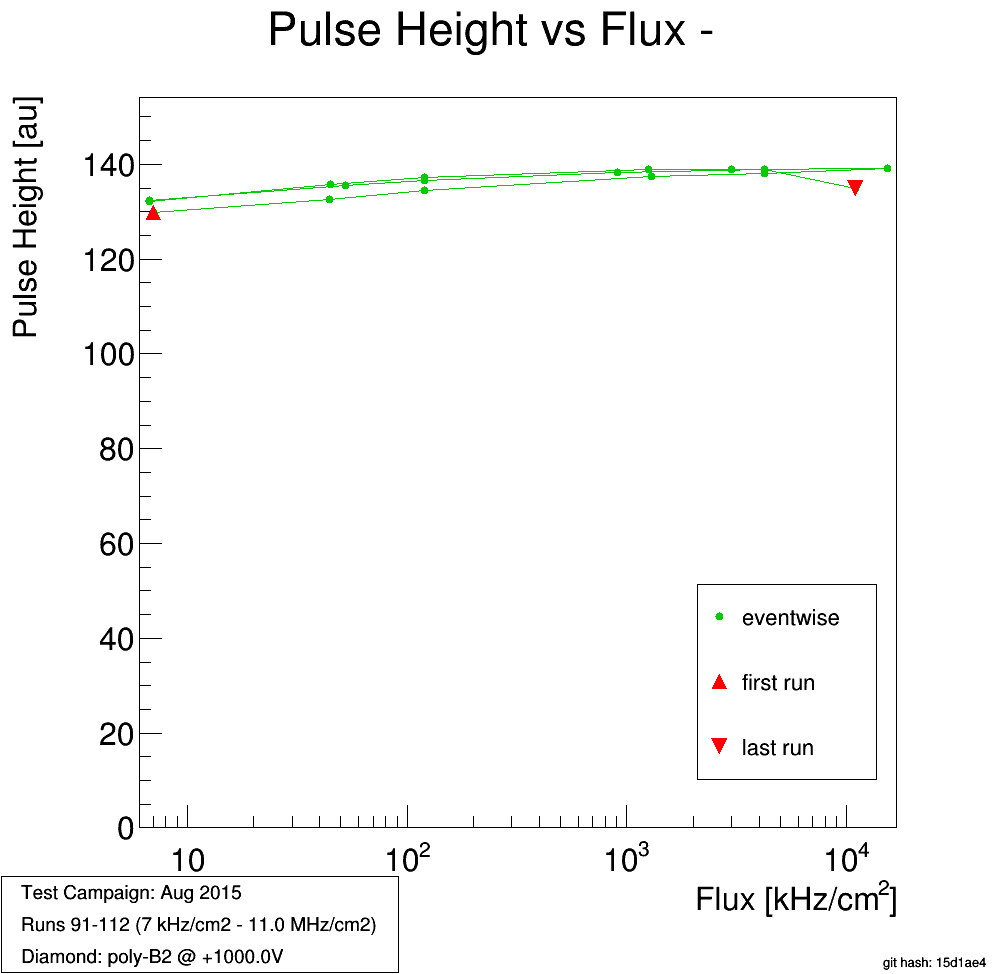
\includegraphics[width=5.5cm]{PhB2PosZero}
	\end{minipage}
\end{frame}
% ====================================================================================
% BEGIN CONCLUSION
% ====================================================================================
\section{Conclusion}
% ============================
\begin{frame}
	\begin{itemize}
		\setlength{\itemsep}{\fill}
		\item exact time sizes of the bins distributed in double gaussian shape around \SI{.5}{ns}
		\item improving signal calculation by fixing the integral in time
		\item general dependence on trigger cell not completeley cured by tcal correction of the DRS4
		\item adding time correction based on remaining dependce on trigger cell
		\item introducing new cut on exact signal peak timing 
		\item secondary beam bunches equally filled
		\item possibly a second particle type in the data
		\item flux measurement yields a good estimation
		\item August data of unirradiated II6-B2 shows stronger dependence on Rate
	\end{itemize}
\end{frame}
% END
% DOCUMENT END
\end{document}

